% !TeX program = xelatex
\documentclass[12pt, a4paper]{article}

%% ── שפה ו-RTL ────────────────────────────────────────────────
\usepackage{fontspec}
% Fix: bidi (loaded by polyglossia) calls \UseMathForPositioningText which is
% undefined in TeX Live 2023+. Define it as a no-op before polyglossia loads bidi.
\providecommand{\UseMathForPositioningText}{}
\usepackage{polyglossia}
\setmainlanguage{hebrew}
\setotherlanguage{english}
\setmainfont{FreeSerif}
\setsansfont{FreeSans}
\setmonofont{FreeMono}

%% ── עמוד ─────────────────────────────────────────────────────
\usepackage{geometry}
\geometry{a4paper, top=2.5cm, bottom=2.5cm, left=2cm, right=3cm}
\usepackage{parskip}
\setlength{\parskip}{6pt}

%% ── מתמטיקה ─────────────────────────────────────────────────
\usepackage{amsmath, amssymb}

%% ── טבלאות ──────────────────────────────────────────────────
\usepackage{booktabs}
\usepackage{array}
\usepackage{longtable}
\usepackage{tabularx}
\usepackage{multirow}

%% ── תמונות ──────────────────────────────────────────────────
\usepackage{graphicx}
\graphicspath{{charts/}}
\usepackage{float}
\usepackage{caption}
\captionsetup{font=small, labelfont=bf}

%% ── קוד ─────────────────────────────────────────────────────
\usepackage{listings}
\usepackage{xcolor}
\lstdefinestyle{pipeline}{
  basicstyle=\ttfamily\small,
  breaklines=true,
  frame=single,
  backgroundcolor=\color{gray!8},
  rulecolor=\color{gray!50},
  xleftmargin=8pt,
  xrightmargin=8pt,
}

%% ── קישורים ─────────────────────────────────────────────────
\usepackage{hyperref}
\hypersetup{
  colorlinks=true,
  linkcolor=blue!70!black,
  urlcolor=cyan!80!black,
  citecolor=green!60!black,
}

%% ── כותרת ───────────────────────────────────────────────────
\title{%
  \textbf{סיכום מחקר --- ModularRAG Optimization}\\[0.5em]
  \large מוטיבציה, שלבי ניסויים, תוצאות ומסקנות
}
\author{Bar Damri}
\date{אוגוסט 2026}

\begin{document}
\maketitle
\tableofcontents
\newpage

%%=============================================================
\section{מוטיבציה ורקע}
%%=============================================================

\subsection{מהי בעיית RAG?}

\textenglish{RAG (Retrieval-Augmented Generation)} הוא ארכיטקטורה שמאפשרת ל-\textenglish{LLM} לענות על שאלות מתוך מאגר גדול של מסמכים. הרעיון בשני שלבים:

\begin{english}
\begin{center}
\texttt{Query\ $\to$\ [Retriever]\ $\to$\ Relevant Docs\ $\to$\ [LLM]\ $\to$\ Answer}
\end{center}
\end{english}

\textbf{הבעיה:} הריטריבר --- הרכיב שמחפש את המסמכים --- טועה בחלק מהמקרים. כשהמסמך הנכון לא מגיע ל-\textenglish{LLM}, התשובה לא יכולה להיות נכונה. אין מנגנון אוטומטי לתיקון שגיאות הריטריבר.

\subsection{הרעיון המנחה --- גישת הטרילטרציה}

הרעיון שהנחה את המחקר הוא אלגוריתם חיפוש איטרטיבי שנקרא \textbf{טרילטרציה} (\textenglish{Trilateration}), בהשראת מיקום \textenglish{GPS}:

\begin{itemize}
  \item ב-\textenglish{GPS}, נקודת המיקום נחשבת מתוך מרחקים לשלושה לווינים.
  \item ברעיון שלנו: אם ל-\textenglish{LLM} יש ``הבנה'' של מרחק סמנטי, ניתן להשתמש בציוניו כדי לחשב ``מרכז כובד'' (\textenglish{centroid}) של מסמכים רלוונטיים ולחפש ממנו מסמכים קרובים יותר בוקטור-\textenglish{DB}.
\end{itemize}

\textbf{התנאי ההכרחי:} ציוני ה-\textenglish{LLM} חייבים לשקף את המרחק האמיתי במרחב האמבדינג. מסמך שה-\textenglish{LLM} מדרג כרלוונטי יותר --- חייב להיות גם קרוב יותר ל-\textenglish{GT} מבחינה גיאומטרית.

\begin{center}
\large\textbf{שאלת המחקר המרכזית:} האם \textenglish{LLM} כ-\textenglish{judge} משקף את הגיאומטריה של מרחב האמבדינג?
\end{center}

%%=============================================================
\section{מונחים מרכזיים}
%%=============================================================

\begin{table}[H]
\centering
\caption{מונחים מרכזיים}
\begin{tabular}{>{\bfseries}rp{10cm}}
\toprule
מונח & הסבר \\
\midrule
\textenglish{GT (Ground Truth)}
  & המסמך הנכון לשאילתה. לכל שאילתה מסמך אחד שמכיל את התשובה הידועה. \\[4pt]
\textenglish{Retriever}
  & הרכיב שמחפש מסמכים רלוונטיים. בפרויקט: \textenglish{Chroma Vector DB} עם \textenglish{cosine similarity}. \\[4pt]
\textenglish{Embedding}
  & ייצוג מספרי (וקטור) של טקסט. מסמכים בעלי תוכן דומה מקבלים וקטורים קרובים זה לזה. \\[4pt]
\textenglish{dist\_to\_gt}
  & מרחק קוסינוס בין אמבדינג מסמך לאמבדינג ה-\textenglish{GT}. $0$ = זהה ל-\textenglish{GT}, $1$ = רחוק לחלוטין. \\[4pt]
\textenglish{LLM-as-a-judge}
  & שימוש ב-\textenglish{LLM} לדירוג רלוונטיות של זוגות (שאילתה, מסמך). בניסויים: \textenglish{Gemini 2.5 Flash Lite}. \\[4pt]
\textenglish{Pool}
  & אוסף המסמכים שנשלחים ל-\textenglish{LLM} לדירוג. \\[4pt]
\textenglish{Global Pool S}
  & \textenglish{Pool} קבוע של 5{,}026 מסמכים, זהה לכל 199 השאילתות (ראה שלב~4). \\[4pt]
\textenglish{Spearman / Pearson / Kendall}
  & מדדי קורלציה. ערך שלילי ($r < 0$) = ציון \textenglish{LLM} גבוה משקף מסמך קרוב יותר ל-\textenglish{GT}. \\[4pt]
\textenglish{ROC-AUC}
  & מדד הפרדה בינארית (\textenglish{GT} לעומת לא-\textenglish{GT}). $1.0$ = הפרדה מושלמת. \\[4pt]
\textenglish{MRR (Mean Reciprocal Rank)}
  & ממוצע $\frac{1}{\mathrm{rank}_{\mathrm{GT}}}$. אופטימי: \textenglish{GT} ראשון בכל טאי. \textenglish{Tie-corrected}: מקום ממוצע ריאלי. \\[4pt]
\textenglish{rag\_failed}
  & דגל שמסמן שהריטריבר לא שם \textenglish{GT} במקום הראשון; ה-\textenglish{GT} עדיין ב-\textenglish{top-200}. \\[4pt]
\textenglish{Score Quantization}
  & ה-\textenglish{LLM} משתמש בפועל בשישה ערכים בלבד: $0.1,\ 0.2,\ 0.4,\ 0.6,\ 0.8,\ 1.0$. \\[4pt]
\textenglish{Tiebreaker Problem}
  & כשמסמכים רבים מקבלים ציון $1.0$ (כולל \textenglish{GT}), דרוש קריטריון שני לשבירת שוויון. \\[4pt]
\textenglish{Jaccard Overlap}
  & חפיפה בין שתי רשימות. $K{=}5$ \textenglish{Jaccard} = כמה מחמשת הראשונים בשתי הרשימות זהים. \\
\bottomrule
\end{tabular}
\end{table}

%%=============================================================
\section{שלב 0 --- הקמת הבסיס (אוקטובר 2024 -- ינואר 2026)}
%%=============================================================

\subsection{מה נבנה}
\begin{itemize}
  \item מאגר \textenglish{PubMedQA} --- 272{,}000 מסמכים רפואיים.
  \item ריטריבר מבוסס \textenglish{Chroma} (\textenglish{cosine similarity} על \textenglish{Sentence-BERT embeddings}).
  \item \textenglish{Pipeline} ראשוני: \textenglish{embed + store + query} $\to$ \textenglish{top-K retrieval}.
  \item \textenglish{Dataset} של 199 שאילתות עם \textenglish{GT} ידוע לכל שאילתה.
\end{itemize}

\subsection{תוכנית האלגוריתם}
\begin{enumerate}
  \item קבל \textenglish{top-K} מסמכים לשאילתה.
  \item בקש מ-\textenglish{LLM} ציון רלוונטיות לכל זוג (שאילתה, מסמך).
  \item חשב \textenglish{centroid} ממושקל (\textenglish{Weighted Centroid / Metric Least Squares}).
  \item חפש ב-\textenglish{DB} מסמכים קרובים ל-\textenglish{centroid}.
  \item חזור עד ל-\textenglish{GT}.
\end{enumerate}

\subsection{מה לא עבד}
ציוני ה-\textenglish{LLM} הראשוניים (סקלה 1--10) היו נמוכים ועקביים --- ה-\textenglish{LLM} לא הצליח להפריד בין מסמכים רלוונטיים ללא-רלוונטיים. נדרשה מתודולוגיה חדשה.

\textbf{מסקנה שהובילה לשלב הבא:} לפני הרצת האלגוריתם, יש לאמת בניסוי ממוקד: האם \textenglish{LLM} מצליח לזהות \textenglish{GT} מתוך קבוצה?

%%=============================================================
\section{שלב 1 --- בדיקת LLM כ-judge (פברואר 2026)}
%%=============================================================

\textbf{עיצוב:} 197 שאילתות. לכל שאילתה --- הציג ל-\textenglish{LLM} את ה-\textenglish{GT} ועוד מסמכים מתחרים ושאל ``מי המסמך הנכון?''

\begin{table}[H]
\centering
\caption{תוצאות שלב~1}
\begin{tabular}{rr}
\toprule
\textbf{מדד} & \textbf{ערך} \\
\midrule
שאילתות שה-\textenglish{LLM} זיהה \textenglish{GT} נכון & 192 / 197 \\
אחוז הצלחה & 97.5\% \\
כישלונות & 5 שאילתות \\
\bottomrule
\end{tabular}
\end{table}

\textbf{פרשנות הכישלונות:} 5 השאילתות שנכשלו נחשדו כ-\textenglish{GT} שגוי בבנצ'מארק עצמו (ה-\textenglish{LLM} בחר מסמך נכון שאינו תואם את ה-\textenglish{GT} הרשמי).

\textbf{מסקנה שהובילה לשלב הבא:} ה-\textenglish{LLM} הוא שופט טוב. אבל השאלה פתוחה: האם ציוניו משקפים מרחב גיאומטרי? יש לבדוק \textbf{קורלציה} בין ציון \textenglish{LLM} ל-\textenglish{dist\_to\_gt}.

%%=============================================================
\section{שלב 2 --- ניסוי קורלציה ראשון, corpus קטן (מאי--יוני 2026)}
%%=============================================================

\subsection{עיצוב ה-Pool}
לכל אחת מ-199 השאילתות, נבנה \textenglish{pool} פרטני:
\begin{itemize}
  \item \textenglish{GT} עצמו.
  \item 100 מסמכים קרובים ביותר ל-\textenglish{GT} (לפי \textenglish{dist\_to\_gt}).
  \item 100 מסמכים קרובים ביותר לשאילתה (ריטריבר).
\end{itemize}
סה"כ $\approx$200 מסמכים לשאילתה, $\approx$1{,}087{,}982 זוגות. ה-\textenglish{LLM} דירג על סקלה 1--10.
\textbf{מאגר:} \textenglish{PubMedQA} --- 272{,}000 מסמכים בלבד.

\subsection{תוצאות עיקריות}

\begin{table}[H]
\centering
\caption{תוצאות ניסוי קורלציה ראשון (272K corpus)}
\begin{tabular}{rr}
\toprule
\textbf{מדד} & \textbf{ערך} \\
\midrule
\textenglish{ROC-AUC} & 0.996 \\
\textenglish{Spearman r} (חציון) & $-0.17$ \\
\textenglish{Pearson r} (חציון) & $-0.39$ \\
דיוק ריטריבר (\textenglish{corpus} 272K) & 95.9\% \\
דיוק \textenglish{LLM} (\textenglish{optimistic P@1}) & 97.4\% \\
\textenglish{MRR optimistic} & 0.98 \\
\textenglish{MRR tie-corrected} & 0.26 \\
\textenglish{MRR pessimistic} & 0.04 \\
\bottomrule
\end{tabular}
\end{table}

\subsection{תגליות מרכזיות}

\paragraph{בעיית הטאי (Tiebreaker Problem)}
ה-\textenglish{LLM} נתן ציון מינימלי (1 בסקלה 1--10) לעשרות מסמכים לא-רלוונטיים --- תיקו מסיבי בתחתית. \textenglish{MRR} ירד מ-$0.98$ (אופטימי) ל-$0.04$ (פסימי).

\paragraph{Hybrid טריוויאלי}
כש-\textenglish{dist\_to\_gt} שימש כ-\textenglish{tiebreaker}, ה-\textenglish{GT} הגיע ראשון ב-100\% מהמקרים. אבל זה טריוויאלי: \textenglish{dist\_to\_gt} של \textenglish{GT} הוא תמיד 0.

\paragraph{בעיית ה-corpus --- ממצא קריטי}
השוואה לספרות מדעית על \textenglish{PubMedQA} (272K):

\begin{table}[H]
\centering
\caption{השוואה לספרות --- 272K corpus}
\begin{tabular}{rr}
\toprule
\textbf{מודל} & \textbf{\textenglish{Recall@K}} \\
\midrule
\textenglish{BM25} & $\approx$67\% \\
\textenglish{BM25 + Contriever} & $\approx$69\% \\
\textenglish{ModernBERT + ColBERT} & $\approx$92.7\% \\
\textbf{ריטריבר שלנו (272K)} & \textbf{95.9\% retrieval / 93.5\% P@1} \\
\bottomrule
\end{tabular}
\end{table}

הדיוק הגבוה אינו הישג --- הוא תוצר של \textenglish{corpus} קטן מדי. ב-272K מסמכים, המסמך הקרוב ביותר לשאילתה הוא כמעט תמיד ה-\textenglish{GT}. עם 25 מיליון מסמכים, התחרות הרבה יותר קשה.

\textbf{מסקנה שהובילה לשלב הבא:} יש להריץ על \textenglish{PubMed} המלא (25M מסמכים) כדי ליצור בנצ'מארק מאתגר אמיתי.

%%=============================================================
\section{שלב 3 --- מסקנת ה-corpus ומעבר ל-PubMed מלא (יוני 2026)}
%%=============================================================

\subsection{החלטות}
\begin{enumerate}
  \item השתמש ב-\textenglish{PubMed} המלא --- 25{,}000{,}000 מסמכים.
  \item לכל שאילתה --- אחזר \textenglish{top-200} מתוך כל 25M.
  \item בנה \textenglish{Pool} גלובלי \textbf{קבוע ומשותף לכל השאילתות} (בניגוד ל-\textenglish{pool} פרטני לכל שאילתה).
  \item הרץ על \textenglish{EC2 GPU} (\textenglish{g4dn.xlarge}) ב-\textenglish{AWS}.
\end{enumerate}

\subsection{רציונל ה-Pool הגלובלי}
שאלה מרכזית שעלתה: למה לקחת לכל שאילתה את המסמכים הקרובים ביותר \emph{אליה}? הרעיון האלגוריתמי (טרילטרציה) מחייב שכל השאילתות יוערכו מול \textbf{אותם מסמכים בדיוק} --- כי \textenglish{Pool} שמשתנה לפי שאילתה מוטה לטובת אותה שאילתה ואינו מדמה תנאי מציאות.

%%=============================================================
\section{שלב 4 --- ניסוי הקורלציה הגלובלי (אוגוסט 2026)}
%%=============================================================

\subsection{ארכיטקטורת הניסוי}

\begin{english}
\begin{lstlisting}[style=pipeline]
25M documents (PubMed)
       |  [EC2 GPU -- embed_and_rank.py]
       v
Top-200 per query  (199 queries)
       |  [build_cross_product.py -- position-by-position interleaving]
       v
Global fixed pool S = 5,026 unique documents
       |
5,026 x 199 = 1,000,174 pairs (query, document)
       |  [Gemini 2.5 Flash Lite via NVIDIA Inference Hub, 80 RPM]
       v
LLM scores 0.0-1.0 per pair
       |
Analysis: correlation, ROC-AUC, MRR, LLM rank
\end{lstlisting}
\end{english}

\subsection{מבנה ה-Pool הגלובלי}
\textenglish{build\_cross\_product.py} ביצע \textenglish{interleaving} לפי מיקום:
\begin{itemize}
  \item מיקום 1: המסמך הראשון של כל שאילתה.
  \item מיקום 2: המסמך השני של כל שאילתה.
  \item וכן הלאה עד מיקום 200.
\end{itemize}
תוצאה: 5{,}026 מסמכים ייחודיים שנבחרו פעם אחת ומשמשים כ-\textenglish{pool} קבוע לכל השאילתות.

\subsection{פרמטרי הרצה}
\begin{itemize}
  \item מודל: \textenglish{Gemini 2.5 Flash Lite} דרך \textenglish{NVIDIA Inference Hub}.
  \item קצב: 80 \textenglish{RPM} עם \textenglish{exponential backoff} ($10\text{s} \to 120\text{s}$, $\pm$25\% \textenglish{jitter}).
  \item זמן הרצה: $\approx$3.5 ימים על מחשב אישי.
\end{itemize}

%%=============================================================
\section{תוצאות מפורטות}
%%=============================================================

\subsection{סטטיסטיקות בסיסיות}

\begin{table}[H]
\centering
\caption{סטטיסטיקות בסיסיות}
\begin{tabular}{rr}
\toprule
\textbf{מדד} & \textbf{ערך} \\
\midrule
זוגות שנוקדו & 1{,}000{,}174 \\
שאילתות עם \textenglish{GT} ידוע ב-\textenglish{DB} & 187 \\
שאילתות ללא \textenglish{GT} ידוע & 12 \\
גודל \textenglish{Pool} (מסמכים ייחודיים) & 5{,}026 \\
ממוצע ציון \textenglish{LLM} (כל הזוגות) & 0.1515 \\
ממוצע \textenglish{dist\_to\_gt} (כל הזוגות) & 0.8682 \\
\bottomrule
\end{tabular}
\end{table}

\subsection{דיוק הריטריבר --- PubMed מלא}

\begin{table}[H]
\centering
\caption{דיוק ריטריבר על 25M corpus}
\begin{tabular}{rr}
\toprule
\textbf{מדד} & \textbf{ערך} \\
\midrule
\textenglish{GT} ב-\textenglish{rank 1} (הצלחה) & 138 / 187 שאילתות \\
\textbf{דיוק ריטריבר P@1} & \textbf{73.8\%} \\
\textenglish{GT} לא ב-\textenglish{rank 1} (כישלון) & 49 / 187 שאילתות \\
שיעור כישלון & 26.2\% \\
\bottomrule
\end{tabular}
\end{table}

\begin{figure}[H]
\centering
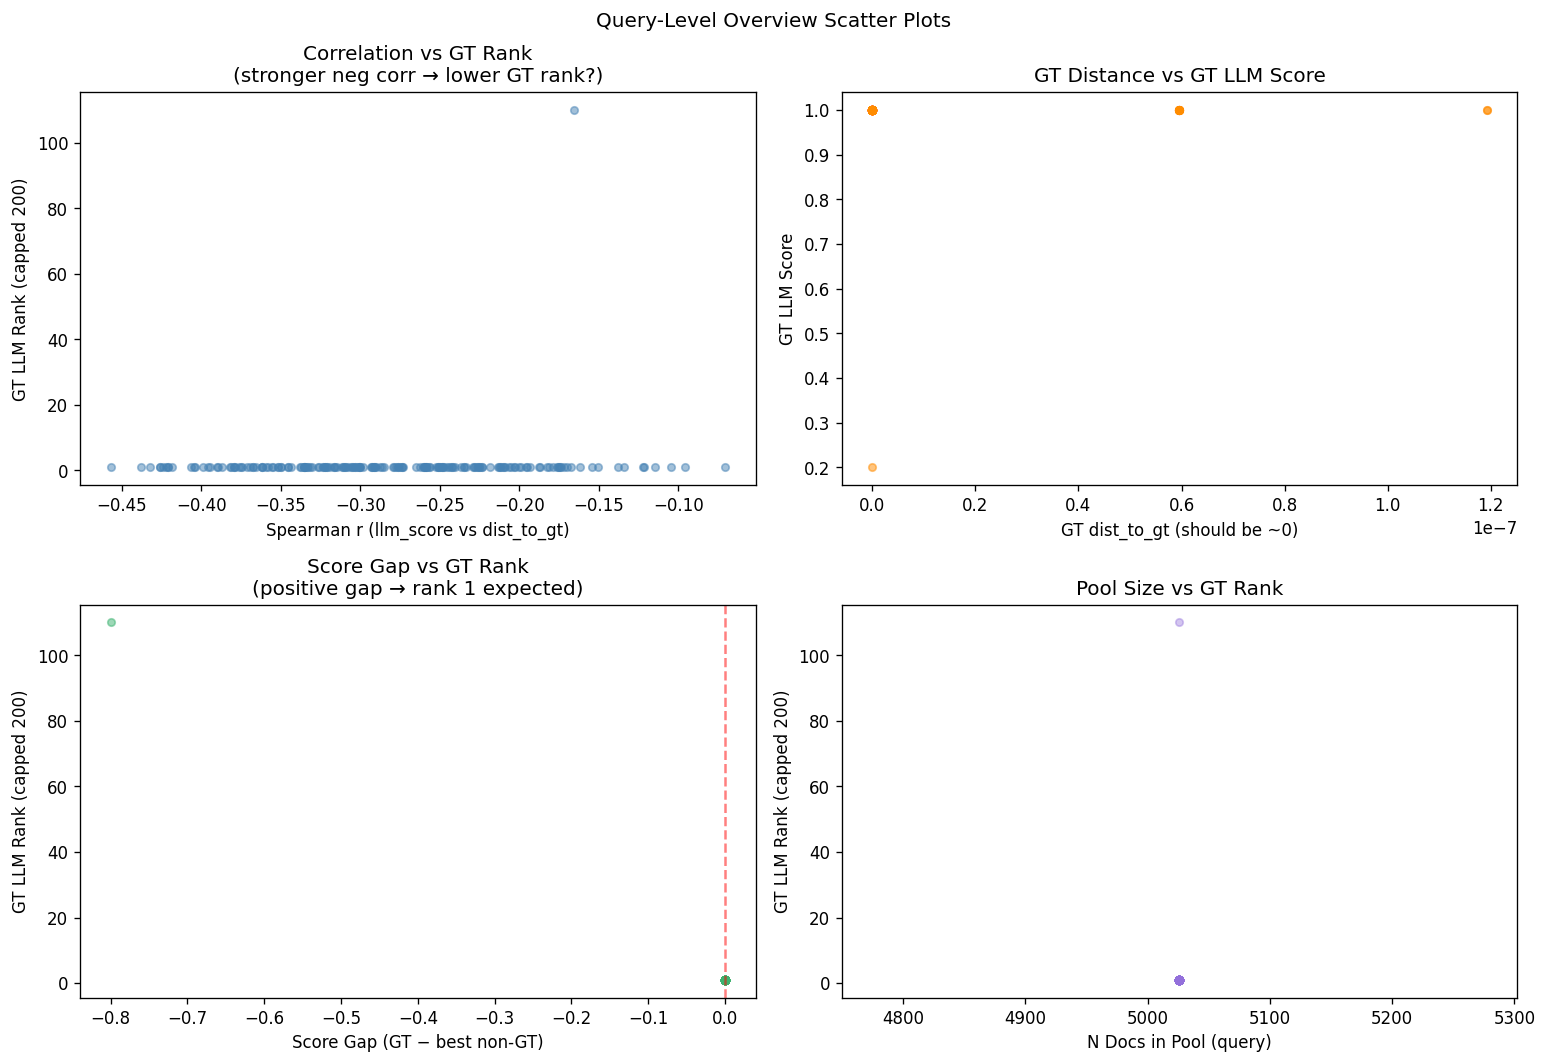
\includegraphics[width=0.95\textwidth]{query_level_overview.png}
\caption{סקירת שאילתות --- ריטריבר מול \textenglish{LLM} לפי שאילתה}
\end{figure}

\textbf{הערה חשובה:} \textenglish{rag\_failed=1} אינו אומר ש-\textenglish{GT} נעדר מה-\textenglish{top-200}. ב-49 השאילתות שנכשלו, ה-\textenglish{GT} נמצא בתוך ה-\textenglish{top-200} (מקום 2 עד 22, ממוצע מקום 5) --- הריטריבר פשוט לא שם אותו ראשון. דיוק 73.8\% על 25M מסמכים מתיישב היטב עם תוצאות ספרות \textenglish{PubMed}.

\subsection{קורלציה --- השאלה המרכזית}

\begin{center}
\textbf{האם ציון \textenglish{LLM} גבוה = מסמך קרוב יותר ל-\textenglish{GT}?}
\end{center}

\begin{table}[H]
\centering
\caption{תוצאות קורלציה על 187 שאילתות}
\begin{tabular}{rrrrrr}
\toprule
\textbf{מדד} & \textbf{חציון} & \textbf{ממוצע} & \textbf{\% שלילי} & \textbf{\% מובהק ($p{<}0.05$)} & \textbf{סימן צפוי} \\
\midrule
\textenglish{Spearman r} & $-0.290$ & $-0.283$ & 100\% & 100\% & שלילי \\
\textenglish{Pearson r}  & $-0.503$ & $-0.494$ & 100\% & 100\% & שלילי \\
\textenglish{Kendall}~$\tau$ & $-0.232$ & $-0.227$ & 100\% & 100\% & שלילי \\
\textenglish{Point-biserial r} & $+0.119$ & $+0.121$ & 0\%   & 99.5\% & חיובי \\
\bottomrule
\end{tabular}
\end{table}

\begin{table}[H]
\centering
\caption{מובהקות סטטיסטית}
\begin{tabular}{rrr}
\toprule
\textbf{מדד} & \textbf{$p$ חציוני} & \textbf{$p$ מקסימלי (הגרוע ביותר)} \\
\midrule
\textenglish{Spearman} & $\sim 10^{-98}$ & $5.18 \times 10^{-7}$ \\
\textenglish{Pearson}  & $\sim 10^{-320}$ & $0.0$ (הצפה מספרית) \\
\bottomrule
\end{tabular}
\end{table}

ה-$p$ הגרוע ביותר ($5.18 \times 10^{-7}$) מובהק בהפרש עצום מעל הסף הקלאסי ($0.05$). 89 מתוך 187 שאילתות מחזירות $p = 0.0$ עבור \textenglish{Pearson} --- הצפה מספרית (הערך האמיתי נמוך מ-$10^{-322}$).

\begin{figure}[H]
\centering
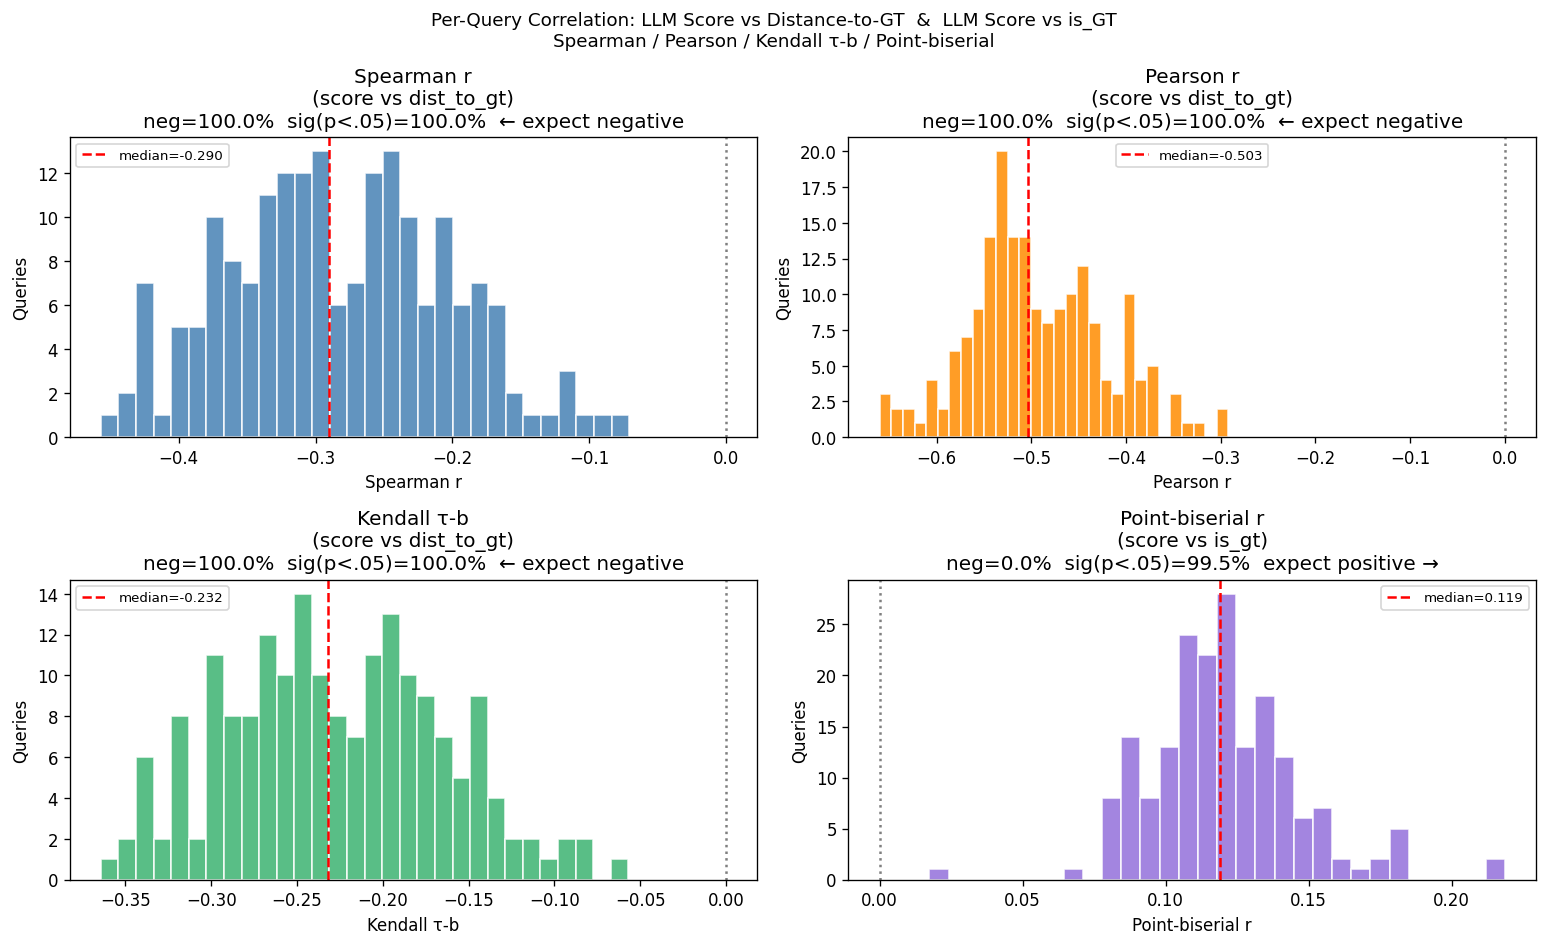
\includegraphics[width=\textwidth]{correlation_histograms.png}
\caption{היסטוגרמות קורלציה --- \textenglish{Spearman}, \textenglish{Pearson}, \textenglish{Kendall} על 187 שאילתות}
\end{figure}

\begin{figure}[H]
\centering
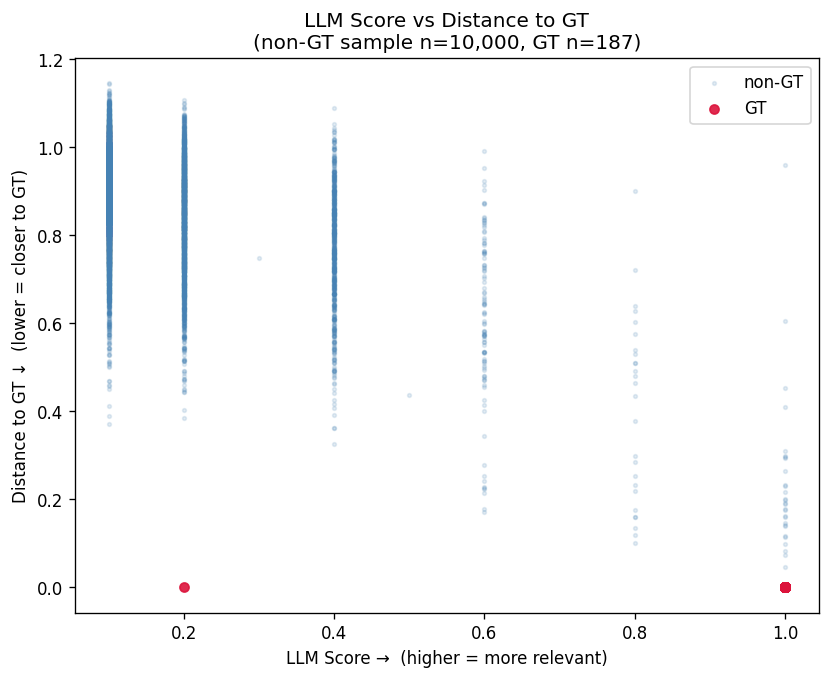
\includegraphics[width=0.9\textwidth]{scatter_score_vs_dist.png}
\caption{פיזור ציון \textenglish{LLM} מול \textenglish{dist\_to\_gt}}
\end{figure}

\begin{figure}[H]
\centering
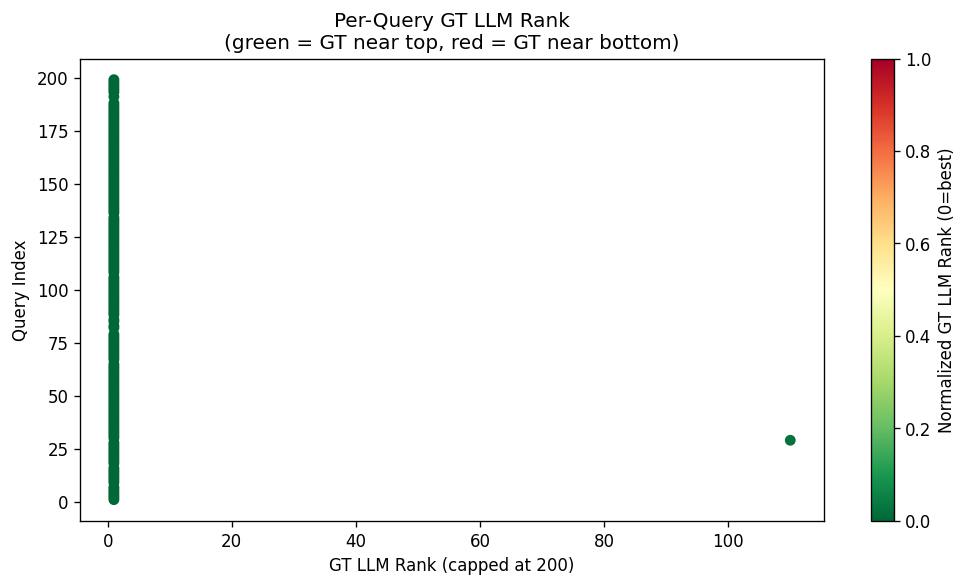
\includegraphics[width=0.9\textwidth]{per_query_gt_rank_scatter.png}
\caption{קורלציה ודירוג \textenglish{GT} לפי שאילתה}
\end{figure}

\subsection{ה-LLM כמזהה GT --- ROC-AUC}

\begin{table}[H]
\centering
\caption{\textenglish{ROC-AUC} ומדדי הפרדה}
\begin{tabular}{rr}
\toprule
\textbf{מדד} & \textbf{ערך} \\
\midrule
\textbf{\textenglish{ROC-AUC}} & \textbf{0.9974} \\
\textenglish{Average Precision (PR-AUC)} & 0.0546 \\
\textenglish{Baseline} אקראי (\textenglish{PR}) & 0.000187 \\
\bottomrule
\end{tabular}
\end{table}

\textenglish{ROC-AUC} של 0.9974 אומר שה-\textenglish{LLM} מצליח להפריד בין ה-\textenglish{GT} לשאר המסמכים בדיוק כמעט מושלם. ה-\textenglish{PR-AUC} הנמוך (0.0546) משקף את האי-איזון הקיצוני: 187 מסמכי \textenglish{GT} מול 999{,}987 לא-\textenglish{GT}.

\begin{figure}[H]
\centering
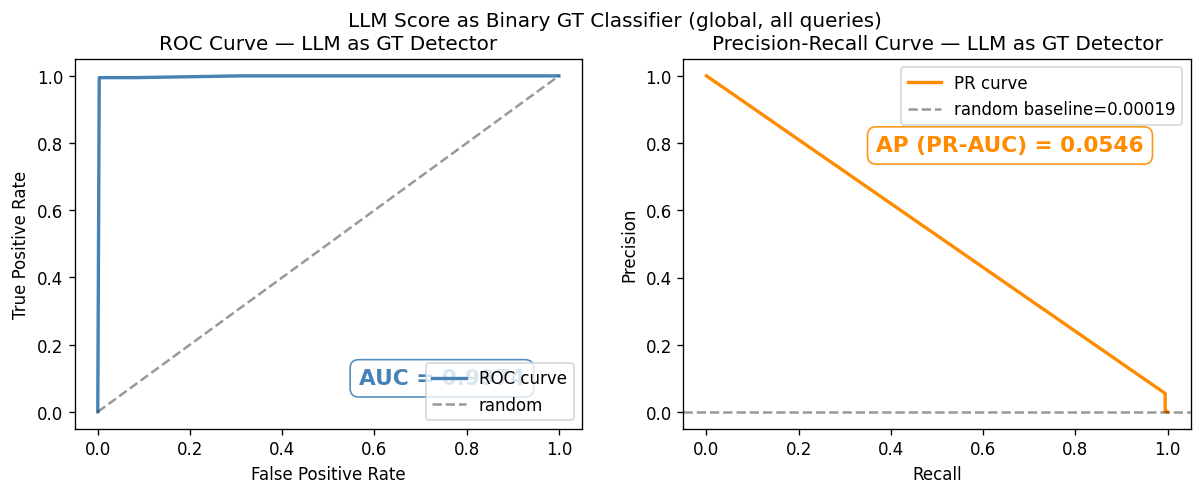
\includegraphics[width=0.9\textwidth]{roc_pr_curves.png}
\caption{\textenglish{ROC} ו-\textenglish{PR Curves}}
\end{figure}

\subsection{התפלגות ציונים}

\begin{table}[H]
\centering
\caption{ציוני \textenglish{GT} לעומת לא-\textenglish{GT}}
\begin{tabular}{rrrrr}
\toprule
\textbf{קבוצה} & \textbf{ספירה} & \textbf{ממוצע} & \textbf{חציון} & \textbf{\textenglish{std}} \\
\midrule
\textenglish{GT}     & 187        & 0.9957 & 1.0 & 0.0585 \\
\textenglish{Non-GT} & 999{,}987  & 0.1513 & 0.1 & 0.1070 \\
\bottomrule
\end{tabular}
\end{table}

\begin{table}[H]
\centering
\caption{פריסת ציונים של \textenglish{Non-GT} --- כימות (\textenglish{Quantization})}
\begin{tabular}{rrr}
\toprule
\textbf{ציון} & \textbf{ספירה} & \textbf{אחוז} \\
\midrule
0.1 & 688{,}097 & 68.8\% \\
0.2 & 235{,}253 & 23.5\% \\
0.4 &  61{,}378 &  6.1\% \\
0.6 &   9{,}256 &  0.93\% \\
0.8 &   2{,}629 &  0.26\% \\
1.0 &   3{,}200 &  0.32\% \\
0.3 / 0.5 / 0.7 / 0.9 & 174 & $<0.02$\% \\
\bottomrule
\end{tabular}
\end{table}

ה-\textenglish{LLM} משתמש בפועל ב-6 ערכים בלבד. 92.3\% מהמסמכים הלא-\textenglish{GT} מקבלים ציון 0.1 או 0.2. האחוזון החציוני של ה-\textenglish{GT} הוא 99.8 --- כלומר ה-\textenglish{GT} נמצא ב-0.2\% העליונים בכל שאילתה.

\begin{figure}[H]
\centering
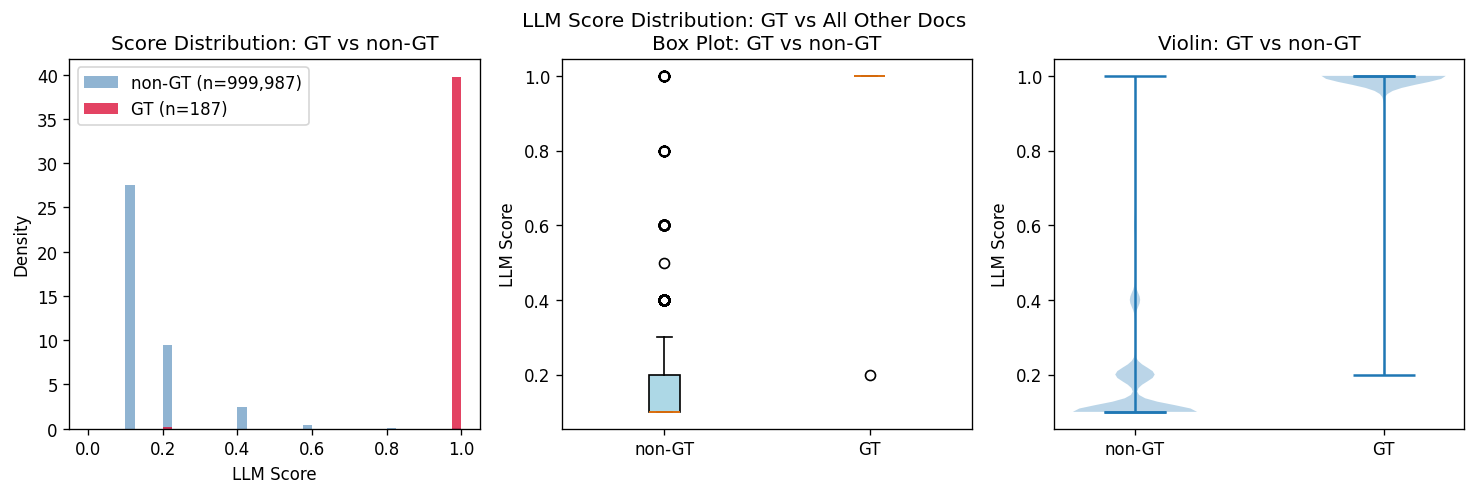
\includegraphics[width=0.9\textwidth]{score_distributions.png}
\caption{התפלגות ציונים --- \textenglish{GT} לעומת \textenglish{Non-GT}}
\end{figure}

\begin{figure}[H]
\centering
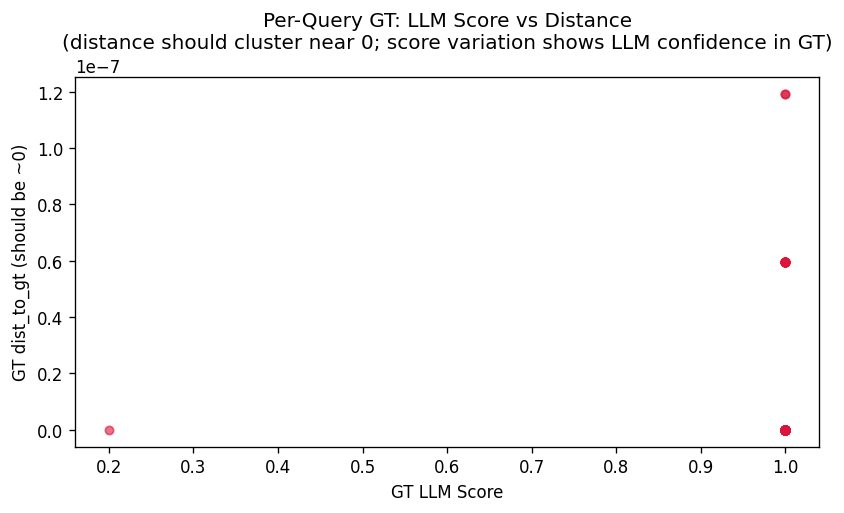
\includegraphics[width=0.9\textwidth]{gt_score_vs_dist.png}
\caption{ציון \textenglish{GT} מול \textenglish{dist\_to\_gt}}
\end{figure}

\begin{figure}[H]
\centering
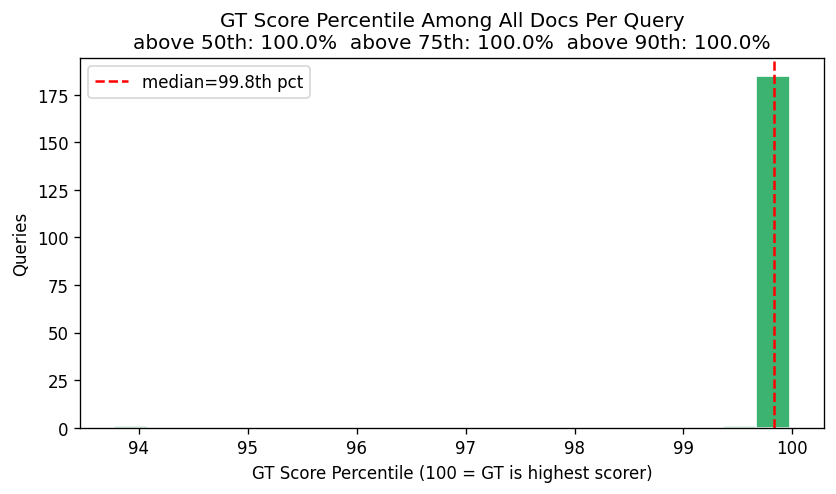
\includegraphics[width=0.9\textwidth]{gt_score_percentile.png}
\caption{אחוזון ציון \textenglish{GT} לפי שאילתה (100 = ציון הגבוה ביותר)}
\end{figure}

\begin{figure}[H]
\centering
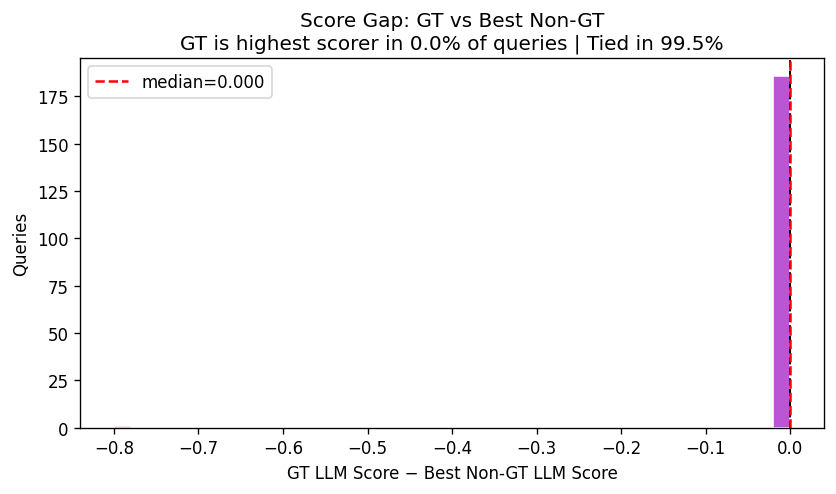
\includegraphics[width=0.9\textwidth]{score_gap.png}
\caption{פער ציון --- \textenglish{GT} לעומת המסמך הטוב ביותר שאינו \textenglish{GT}}
\end{figure}

\subsection{דירוג GT ע"י LLM}

\begin{table}[H]
\centering
\caption{דירוג \textenglish{GT} ע"י \textenglish{LLM}}
\begin{tabular}{rr}
\toprule
\textbf{מדד} & \textbf{ערך} \\
\midrule
\textbf{\textenglish{MRR} (אופטימי --- \textenglish{ties = rank 1})} & \textbf{0.9947} \\
\textbf{\textenglish{P@1} (אופטימי)} & \textbf{99.5\% (186/187)} \\
\textenglish{MRR} (\textenglish{tie-corrected}) & 0.1348 \\
\textenglish{P@1} (\textenglish{tie-corrected}) & 0.0\% \\
\bottomrule
\end{tabular}
\end{table}

\begin{itemize}
  \item \textbf{\textenglish{Optimistic P@1} = 99.5\%:} \textenglish{GT} מקבל ציון 1.0 ב-186/187 שאילתות.
  \item \textbf{\textenglish{Tie-corrected P@1} = 0\%:} ב-186 מהמקרים, עוד מסמכים קיבלו ציון 1.0. מספר חציוני $\approx$18 מסמכים במקום הראשון.
  \item \textbf{הכישלון היחיד (שאילתה 29):} \textenglish{GT} קיבל ציון 0.2 ודורג במקום 110 מתוך 5{,}026 --- המקרה היחיד שבו ה-\textenglish{LLM} לא זיהה את ה-\textenglish{GT}.
\end{itemize}

\begin{figure}[H]
\centering
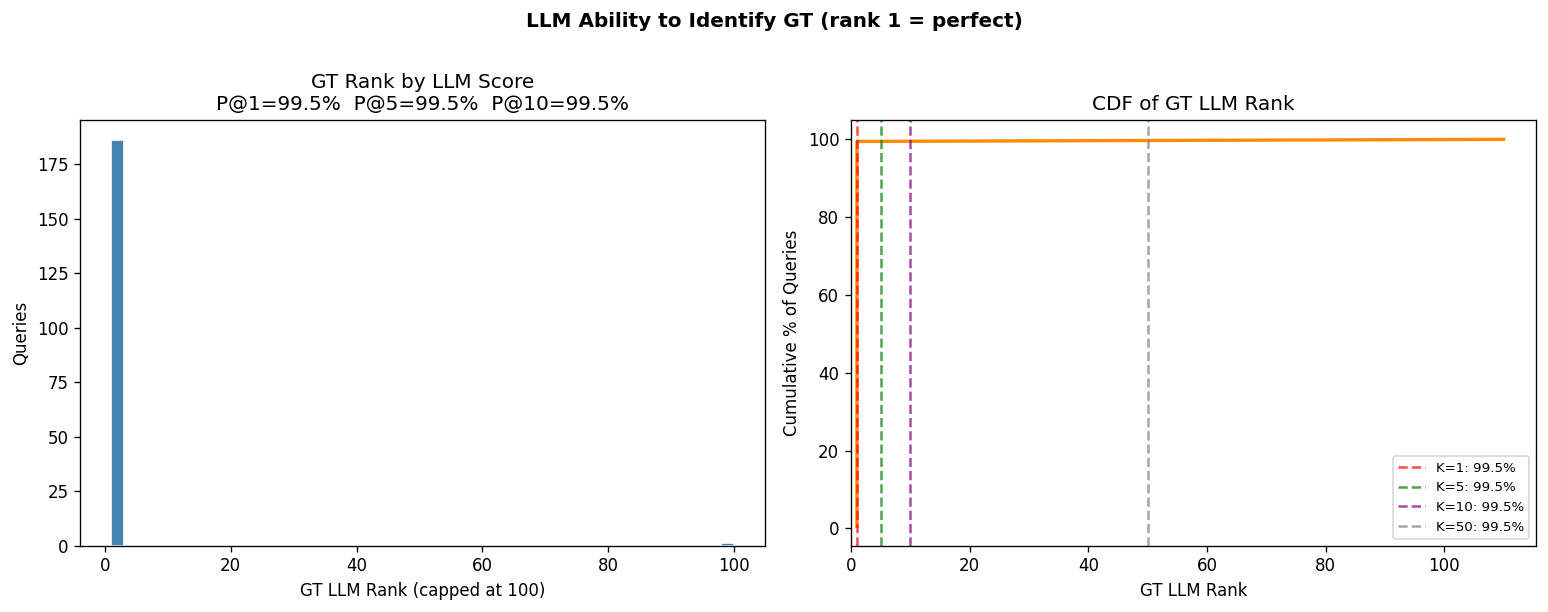
\includegraphics[width=0.9\textwidth]{gt_llm_rank.png}
\caption{דירוג \textenglish{GT} ע"י \textenglish{LLM} לפי שאילתה}
\end{figure}

\subsection{ניתוח ``הצלת'' הריטריבר ע"י LLM}

ב-49 השאילתות שהריטריבר נכשל (\textenglish{GT} לא ב-\textenglish{rank 1}), האם ה-\textenglish{LLM} ``מציל'' את המצב?

\begin{table}[H]
\centering
\caption{ניתוח הצלה --- 49 שאילתות שהריטריבר נכשל בהן}
\begin{tabular}{rr}
\toprule
\textbf{תרחיש} & \textbf{תוצאה} \\
\midrule
\textenglish{LLM} מעניק ל-\textenglish{GT} ציון 1.0 & 49/49 (100\%) \\
\textenglish{LLM} ``מציל'' לוגית (\textenglish{GT} בפסגה משותפת) & 49/49 (100\%) \\
\textbf{הצלה אמיתית (ריטריבר כ-\textenglish{tiebreaker})} & \textbf{4/49 (8.2\%)} \\
\bottomrule
\end{tabular}
\end{table}

\textbf{הסבר הפער:} ב-\textenglish{RAG} אמיתי, כשמסמכים מקבלים אותו ציון \textenglish{LLM} (1.0), דרוש קריטריון שני. אם הריטריבר משמש כ-\textenglish{tiebreaker}, המסמכים שהיו מדורגים לפני ה-\textenglish{GT} ב-\textenglish{retriever} ימשיכו להיות לפניו, כי ה-\textenglish{LLM} לא מבדיל ביניהם.

בממוצע, ה-\textenglish{GT} עלה מ:
\begin{itemize}
  \item מקום ריטריבר ממוצע: \textbf{5.0} (בשאילתות שנכשלו).
  \item מקום \textenglish{LLM} ממוצע: \textbf{$\approx$3.3} (בקבוצת הטאי).
\end{itemize}
כלומר ה-\textenglish{LLM} קידם את ה-\textenglish{GT} בממוצע $\approx$1.7 מקומות, אבל לא מספיק כדי להעביר אותו לפסגה ייחודית.

\begin{figure}[H]
\centering
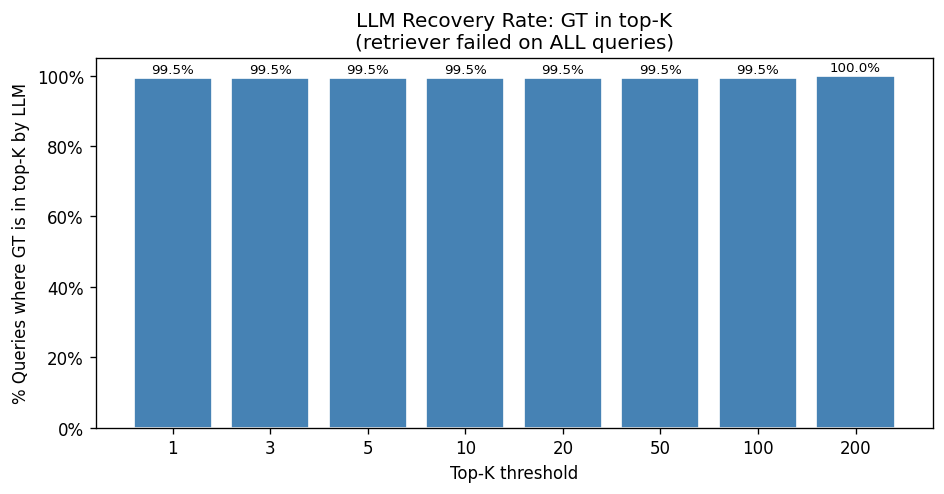
\includegraphics[width=0.9\textwidth]{llm_recovery_at_k.png}
\caption{\textenglish{LLM Recovery at K} --- שיעור השאילתות שבהן \textenglish{GT} נמצא ב-\textenglish{Top-K}}
\end{figure}

\subsection{ניתוח קוונטיל מרחק}

\begin{table}[H]
\centering
\caption{ציון \textenglish{LLM} ממוצע לפי בין מרחק ל-\textenglish{GT}}
\begin{tabular}{rrr}
\toprule
\textbf{בין (\textenglish{dist\_to\_gt})} & \textbf{ציון ממוצע} & \textbf{מסמכים} \\
\midrule
הכי קרוב (0.022--0.718) & \textbf{0.271} & 99{,}999 \\
(0.718--0.785) & 0.171 & 99{,}999 \\
(0.785--0.827) & 0.153 & 99{,}998 \\
(0.827--0.859) & 0.144 & 100{,}000 \\
(0.859--0.886) & 0.138 & 99{,}998 \\
(0.886--0.912) & 0.133 & 99{,}998 \\
(0.912--0.938) & 0.130 & 99{,}999 \\
(0.938--0.965) & 0.126 & 99{,}998 \\
(0.965--1.0)   & 0.124 & 99{,}999 \\
הכי רחוק (1.0--1.207) & 0.122 & 99{,}999 \\
\bottomrule
\end{tabular}
\end{table}

ציון \textenglish{LLM} יורד בצורה \textbf{מונוטונית} ככל שהמסמך רחוק יותר מה-\textenglish{GT} --- אימות ישיר לקורלציה.

\begin{figure}[H]
\centering
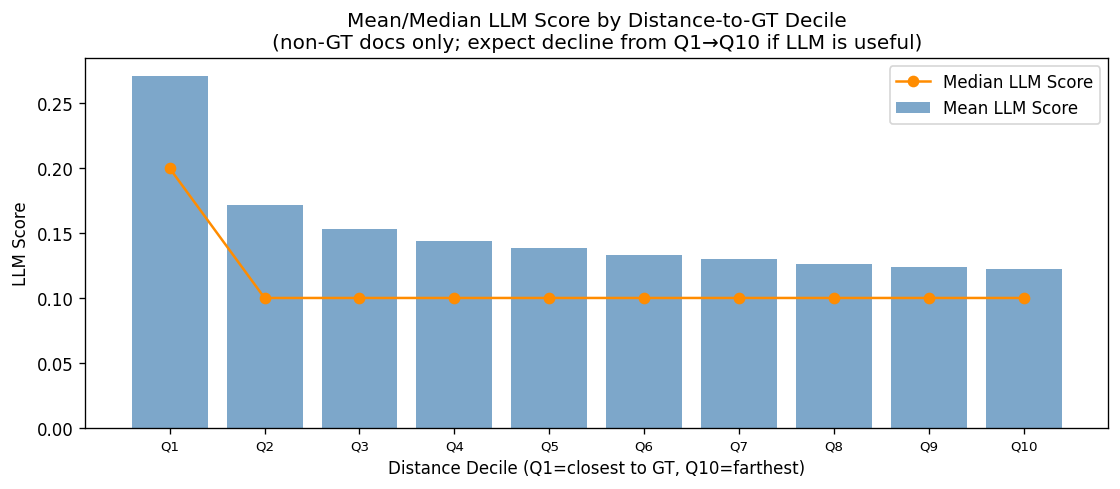
\includegraphics[width=0.9\textwidth]{distance_quantile_analysis.png}
\caption{ניתוח קוונטיל מרחק --- ציון ממוצע לפי בין מרחק ל-\textenglish{GT}}
\end{figure}

\begin{figure}[H]
\centering
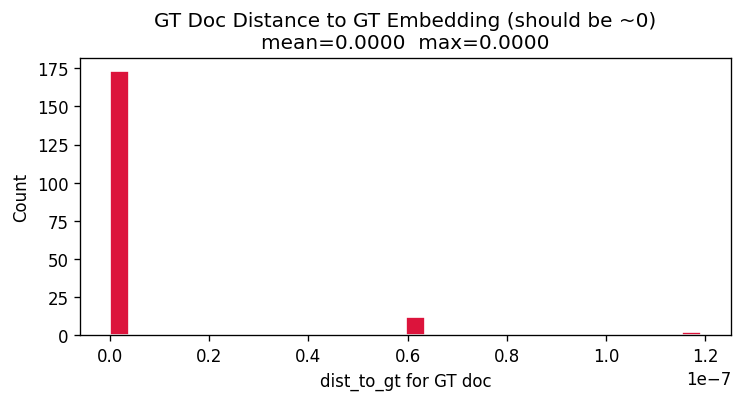
\includegraphics[width=0.9\textwidth]{gt_dist_sanity.png}
\caption{בדיקת שפיות --- מרחק \textenglish{GT} בתוך ה-\textenglish{Pool}}
\end{figure}

\subsection{Jaccard Overlap --- query-space לעומת GT-space}

\begin{table}[H]
\centering
\caption{\textenglish{Jaccard Overlap} בין \textenglish{top-K} של שאילתה ל-\textenglish{top-K} של \textenglish{GT}}
\begin{tabular}{rrr}
\toprule
\textbf{K} & \textbf{\textenglish{Jaccard} חציוני} & \textbf{פרשנות} \\
\midrule
5   & 0.25 & 1--2 מסמכים משותפים מבין 5 \\
10  & 0.33 & $\approx$3 מסמכים משותפים מבין 10 \\
20  & 0.60 & 12 מסמכים משותפים מבין 20 \\
50  & 0.37 & 18--19 מסמכים משותפים מבין 50 \\
100 & 0.26 & $\approx$26 מסמכים משותפים מבין 100 \\
\bottomrule
\end{tabular}
\end{table}

\textenglish{Top-5} של שאילתה ו-\textenglish{Top-5} של \textenglish{GT} חופפים בממוצע 25\% בלבד. שני האמבדינגים מצביעים על אזורים שונים במרחב --- זו סיבה ישירה לכישלונות הריטריבר.

\begin{figure}[H]
\centering
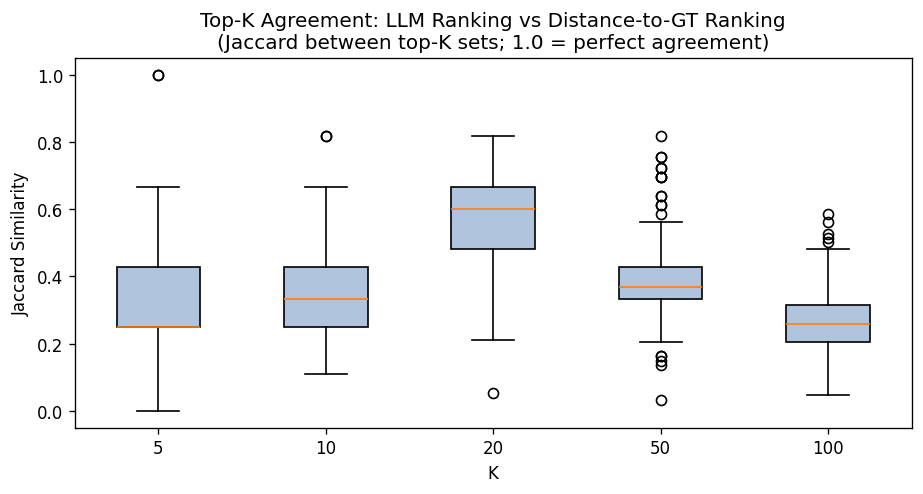
\includegraphics[width=0.9\textwidth]{topk_jaccard.png}
\caption{\textenglish{Top-K Jaccard Overlap} --- \textenglish{query-space} לעומת \textenglish{GT-space}}
\end{figure}

%%=============================================================
\section{מסקנות ומשמעות}
%%=============================================================

\subsection{מה הוכח?}

\textbf{התנאי ההכרחי לאלגוריתם הטרילטרציה מתקיים:}
\begin{itemize}
  \item קורלציה שלילית ב-100\% מהשאילתות, $p < 10^{-7}$ בכל מקרה.
  \item ה-\textenglish{LLM} אכן משקף מרחקים גיאומטריים במרחב האמבדינג.
  \item \textenglish{ROC-AUC} של 0.9974 --- ה-\textenglish{LLM} מזהה \textenglish{GT} בדיוק גבוה מאוד.
\end{itemize}

\textbf{ה-\textenglish{LLM} כ-\textenglish{filter} גס --- מצוין. ה-\textenglish{LLM} כ-\textenglish{ranker} עדין --- לא מספיק:}
\begin{itemize}
  \item הסטורציה ל-1.0 מונעת הפרדה בתוך הטייר העליון.
  \item $\approx$18 מסמכים בממוצע מקבלים ציון 1.0 יחד עם ה-\textenglish{GT}.
\end{itemize}

\subsection{מה עדיין חסר?}

\begin{table}[H]
\centering
\caption{אתגרים פתוחים והצעות לפתרון}
\begin{tabular}{rp{8cm}}
\toprule
\textbf{אתגר} & \textbf{הצעה לפתרון} \\
\midrule
\textenglish{Tiebreaker} בתוך ציון 1.0 & \textenglish{Cross-encoder} (ציון רציף מדויק) \\
ציוני \textenglish{LLM} גסים (6 ערכים) & \textenglish{Prompt} שמבקש הסברים מספריים רציפים \\
26.2\% כישלון ריטריבר & אלגוריתם טרילטרציה עם \textenglish{Pool} מתחדש \\
\bottomrule
\end{tabular}
\end{table}

\subsection{השוואת שלבים}

\begin{table}[H]
\centering
\caption{השוואה בין שלבי הניסויים}
\begin{tabular}{rrrrrr}
\toprule
\textbf{שלב} & \textbf{\textenglish{Corpus}} & \textbf{\textenglish{Pool}} & \textbf{\textenglish{Retriever P@1}} & \textbf{\textenglish{ROC-AUC}} & \textbf{\textenglish{Spearman r}} \\
\midrule
ניסוי קורלציה ראשון & 272K & פרטני & 95.9\% & 0.996  & $-0.17$ \\
\textbf{ניסוי גלובלי (שלב~4)} & \textbf{25M} & \textbf{גלובלי} & \textbf{73.8\%} & \textbf{0.9974} & $\mathbf{-0.290}$ \\
\bottomrule
\end{tabular}
\end{table}

עם \textenglish{corpus} גדול יותר (25M במקום 272K), הריטריבר נכשל יותר (73.8\% לעומת 95.9\%) --- בדיוק כפי שציפינו ותכננו. הקורלציה \textbf{עלתה} (\textenglish{Spearman} $-0.29$ לעומת $-0.17$) --- הגדלת ה-\textenglish{corpus} העמיקה את הקורלציה.

%%=============================================================
\appendix
\section{מיקום קבצים}
%%=============================================================

\begin{english}
\begin{lstlisting}[style=pipeline]
results/cloud_runs/staged_run_2026-08-03_08-32-45/
|-- experiment_results.db          [75 MB, Git LFS]  1,000,174 scored pairs
|-- scoring_queue.parquet          [29 MB]            top-200 per query
|-- expanded_scoring_queue.parquet [768 MB, Git LFS]  full cross-product
|-- run_state.json                                    phase2_complete=true
|-- analysis/
    |-- report_full.html / .pdf    full analysis report
    |-- report_summary.html / .pdf summary report for sharing
    |-- charts/base/               14 PNG charts (copied here as charts/)
    |-- csv/global/                global CSV summaries
    |-- csv/per_query/             per-query CSV data
\end{lstlisting}
\end{english}

\begin{english}
\begin{lstlisting}[style=pipeline]
Key source files:
  embed_and_rank.py        Phase 0: embedding + retrieval over 25M docs (EC2)
  build_cross_product.py   Build global fixed pool S (interleaving)
  score_from_queue.py      Phase 2: LLM scoring via NVIDIA Inference Hub
  utility/llm_gateway.py  Non-blocking dispatcher with exponential backoff
  configurations/config.py NVIDIA IH settings, 80 RPM rate limit
\end{lstlisting}
\end{english}

\bigskip
\begin{center}
\textit{סיכום זה נכתב באוגוסט 2026 ומייצג את מצב המחקר עד לניסוי הגלובלי על \textenglish{PubMed} המלא.}
\end{center}

\end{document}
